\documentclass[border=2pt]{standalone}
\usepackage{tikz}
\begin{document}
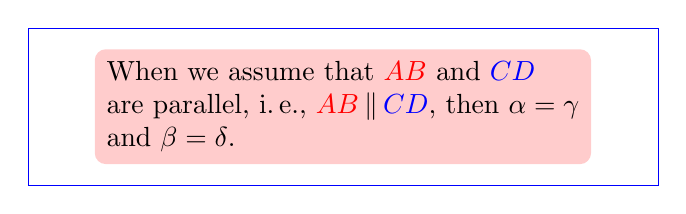
\begin{tikzpicture}
  \draw[blue,line width=.2pt] (-4,-1) rectangle (4,1);
  \node[text width=6cm,rounded corners,fill=red!20,inner sep=1ex]
    {When we assume that $\color{red}AB$ and $\color{blue}CD$ are
     parallel, i.\,e., ${\color{red}AB} \mathbin{\|} \color{blue}CD$,
     then $\alpha=\gamma$ and $\beta=\delta$.};
\end{tikzpicture}
\end{document}
